\documentclass[11pt, conference]{IEEEtran}
\usepackage[spanish]{babel}
\usepackage[utf8]{inputenc}
\usepackage{amsmath}
\usepackage{amsfonts}
\usepackage{cite}
\usepackage{graphicx}

\begin{document}
	\title{\bf Generación de números Primos}
	\author{Universidad Católica San Pablo \\ Kevin Jhomar Sanchez Sanchez}
\onecolumn
\maketitle

\bigskip\bigskip\bigskip\bigskip
\bigskip\bigskip\bigskip\bigskip

\tableofcontents 
\twocolumn
\pagebreak
\section{Introducción}
Dentro del mundo de la criptografia hay números muy especiales, llamados numeros primos, y es en este punto donde comienza nuestra investigacion. 

\

Mostrare como se genera un numero primo fuerte y veremos como es que se prueba que un numero $n$ es un numero primo.

\section{Números primos}
\subsection{Definición}
Un número primo es un número natural mayor que 1, que tiene únicamente dos divisores distintos: él mismo y el 1. 

\

En el campo de teoría de los números hay una parte donde se especializa solo en el estudio de los números primos, en estas ramas se estudian básicamente todas sus propiedades aritméticas.

\

Algo interesante de ver es que si se consideran números individuales, los primos parecen estar distribuidos aleatoriamente, pero la distribución «global» de los números primos sigue leyes bien definidas.

\

\textbf{NOTA:} El número 1, por convenio, no se considera ni primo ni compuesto, y la propiedad de ser primo se denomina \textbf{primalidad}.
\subsection{Generación de primos fuertes}
Un número primo fuerte es un número con las siguientes propiedades.

\

\textbf{Propiedades}
\begin{enumerate}
	\item $p$ es un número primo.
	\item $p-1$ tiene factores primos grandes.\\ Es decir, $p=a_{1}q_{1}+1$ para algún entero $a_{1}$ y un primo grande $q_{1}$.
	\item ${q_{1}-1}$ tiene factores primos grandes.\\ Es decir,$q_{1}=a_{2}q_{2}+1$ para algún entero $a_{2}$ y un primo grande $q_{2}$. 
	\item $p+1$ tiene factores grandes.\\ Es decir $p = a_{3}q_{3}-1$ para algún entero $a_{3}$ y un primo grande $q_{3}$. 

\end{enumerate} 

\

\textbf{Ejemplo.}Si $q_1$ = 11, $a_1$ = 2, entonces lo introducimos a $p=a_{1}q_{1}+1$ y resolviendo  $p$ = 2*11 + 1 = 23.

\subsection{La Primalidad}
La primalidad consiste en determinar, de forma aleatoria, números primos grandes. El problema surge, entre otras razones porque dentro del criptosistema RSA se necesita implementar, dos números primos $p$ y $q$, de longitud grande (de mas de 100 dígitos). 

\

En general, para resolver el problema se recurre a los test de primalidad y pseudoprimalidad, Un test de primalidad es un criterio para decidir si un numero dado es o no primo, que esta dentro de una matriz o dentro de un rango.\cite{a}

\section{Test de Pseudoprimalidad}
\subsection{Teorema de Tchebycheff}
Esta ecuacion fue demostrado en primer lugar por Hadamard y de la Vallée Poussin en 1896 basandose en algunas propiedades de la funcion Zeta de Riemann. 

\

Este teorema calcula la cantidad de números primos menores o iguales que $x$, $\pi(x)$, que es asintoticamente equivalente a $x/ln(x)$, es decir:

	\[
	\lim_{n \to \infty} \frac{\pi(x)}{\frac{x}{ln(x)}}=1
	\]

\textbf{Cuadro grafico del algoritmo}
\begin{figure}[h]
	\begin{center}
		
\includegraphics[scale=0.5]{6.png}
		\caption{Tabla del teorema de Tchebycheff} 
	\end{center}
\end{figure}\\
\textbf{Donde:}
$x$ es el número de bits y $\pi(x)$ es la cantidad de primos que hay en el rango de $x$\\


\subsection{El Pequeño Teorema de Fermat}
Con este teorema se diferenciar a un numero primo de un número compuesto.\cite{c}

\

Donde para todo $p$ que es un número primo.
\begin{enumerate}
	\item Si $MCD(a, p) = 1$, entonces $a^{(p-1)}\equiv1(mod\ p)$ 
	\item Si $r\equiv s(mod\ p-1)$, entonces $a^r\equiv a^{s}(mod\ p)$ para todos los enteros $a$. En otras palabras, cuando se trabaja a un numero primo $p$ los exponentes pueden ser reducidos a $p-1$
	\item De una forma particular $a^p\equiv a(mod\ p)$ para todo entero $a$
\end{enumerate}
\textbf{Ejemplo.} Consideraremos el numero n = 91. Este numero es un pseudoprimo de base b=3, puesto que $3^{90}\equiv 1(mod\ 91)$; sin embargo ,91 no es pseudoprimo de base b = 2, puesto que $2^{90}\equiv 64(mod\ 91)$.
 
\subsection{Teorema de Mersenne}
Si $2^{n}-1$ es primo, entonces $n$ es primo. Si $n$	es primo y $2^{n}-1$, entonces $M_{n}=2^{n}-1$ se llama primo de Mersenne.

No se sabe si existen infinitos primos de Mersenne. El ultimo conocido es $M_{74 207 281}=2^{74 207 281}-1$ de 49 números primos.

\section{Test de Primalidad}
Es un criterio para decidir si un numero dado es o no primo, que esta dentro de una matriz o dentro de un rango. El test de primalidad internamente tiene algoritmos que generalmente se dividen en dos ramas muy claras y estas son:

\begin{enumerate}
	\item \textbf{Algoritmos deterministas}. son algoritmos completamente predictivos, donde si de conocen sus entradas, también conoceríamos su salida.
	\item \textbf{Algoritmos probabilistas}. son algoritmos que basan sus resultados en la toma de algunas decisiones al azar, de tal forma que, en promedio, obtiene una buena solución al problema planteado para cualquier distribución de los datos de entrada, claro que se tiene un margen de error al momento de la generación de números primos.
\end{enumerate}

\subsection{Teorema de Wilson}
Este teorema(también llamado Congruencia de Wilson) se enuncia de la siguiente manera.\cite{b}

\begin{center}
	Si $p$ es un numero primo, entonces $(p-1)!\equiv-1(mod\ p)$
\end{center} 

El teorema de Wilson no se utiliza como test de primalidad en la práctica, ya que para calcular $(p-1)!\ mod\ n$ para un número $n$ grande es costoso (computacionalmente hablando), y se conocen test más sencillos y rápidos. Gráficamente podemos verlo de esta manera.

\begin{figure}[h]
	\begin{center}
		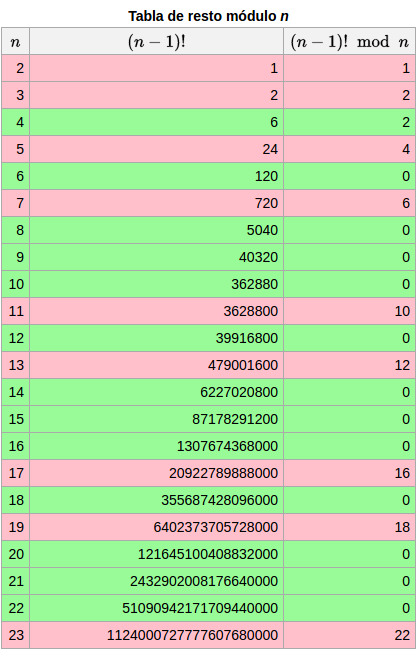
\includegraphics[scale=0.5]{1.png}
		\caption{Tabla del teorema de wilson} 
	\end{center}
\end{figure}

Usando el teorema del Wilson, se tiene que para cada número primo p:

$1\cdot2\cdot\cdot\cdot(p-1)\equiv-1(mod\ p)$

$1\cdot(p-1)\cdot2\cdot(p-2)\cdot\cdot\cdot n\cdot(p-n)\equiv1\cdot(-1)\cdot2\cdot(-2)\cdot\cdot\cdot n\cdot(-n)\equiv-1(mod\ p)$

donde $p=2n+1$. Esto se convierte en:

$\displaystyle\prod_{j=1}^n j^{2}\equiv(-1)^{n+1}\  (mod\ p)$  

o también

$(n!){2}\equiv(-1)^{m+1}\ (mod\ p)$  

El teorema de Wilson ha sido utilizado para generar fórmulas para los primos, pero es demasiado lento como para tener valor práctico.
\subsection{Criba de Eratostenes}
La criba de eratostenes es una algoritmo empleado para hallar números primos menores o igual a un $n$ natural. \cite{e}

\

Comenzando por el número 2 se tachan todos sus múltiplos, en la siguiente iteración se toma el siguiente menor numero de la criba y se tachan todos sus múltiplos y así hasta que el número primo al cuadrado sea mayor al $n$

\begin{figure}[h]
	\begin{center}
		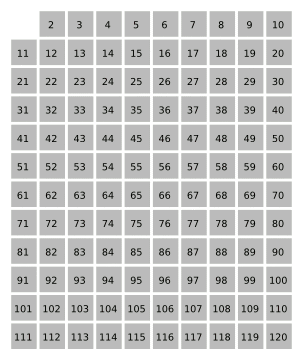
\includegraphics[scale=0.5]{5.png}
		\caption{Criba de eratostenes, donde n=120} 
	\end{center}
\end{figure}

La complejidad Algorítmica de la criba es $O(N\ (log\ log\ N))$, esta complejidad es muy problemática al entender que para números mayores a 20 bits es muy lento(hablando desde un aspecto computacional).

\subsection{Criba de Atkin}
Es un algoritmo diseñado por A.O.L. Atkin y Daniel J. Bernstein es rápido y moderno, empleado para hallar números primos menores o igual a un $n$ natural. 

\

En realidad es una versión mas optimizada de la criba de eratóstenes, pero a diferencia de eratóstenes, este algoritmo realiza trabajos preliminares y no tacha los múltiplos de los números primos como lo hace eratóstenes, sino que mas bien tacha los cuadrados de los primos múltiplos.

\

El algoritmo desde un inicio marca una liste de resultados, que normalmente esta compuesta por 2,3 y 5. También se crea una lista con cada entero positivo y cada casilla debe estar marcado desde un inicio como <<no primo>>. Entonces para cada entrada de la lista de criba se realizan los siguientes pasos:
\begin{enumerate}
	\item Si la entrada es un numero con resto  1, 13, 17, 29, 37, 41, 49 ó 53, se invierte tantas veces como soluciones posibles hay para $4x^{2} + y^{2}$ = entrada
	\item Si la entrada es un número con resto 7, 19, 31 ó 43, se invierte tantas veces como soluciones posibles hay para $3x^{2} + y^{2}$= entrada.
	\item Si la entrada es un número con resto 11, 23, 47 ó 59, se invierte tantas veces como soluciones posibles hay para $3x^{2} - y^{2}$ = entrada con la restricción $x > y$.
	\item Si la entrada tiene otro resto, se ignora.
\end{enumerate}
Después de estos pasos se toma el menor de la lista de la criba y se toma al numero de la lista marcado como primo, después se incluyen el numero en la lista de resultados.
Se eleva el número al cuadrado y se marcan todos los múltiplos de ese cuadrado como <<no primos>>. Después hay que repetir estos últimos pasos.
La complejidad computacional esta dada por
\[O(N/log\ log\ N)\] con solo $N^{1/2+o(1)}$ bits de memoria, lo que lo hace ligeramente mejor que la criba de eratóstenes que su complejidad algorítmica es $O(N^{1/2}(log\ log\ N)/log\ N)$ bits de memoria.

\textbf{De manera mas gráfica podemos verlo así}

\begin{figure}[h]
	\begin{center}
		\[4x^{2}+y^{2}\]
		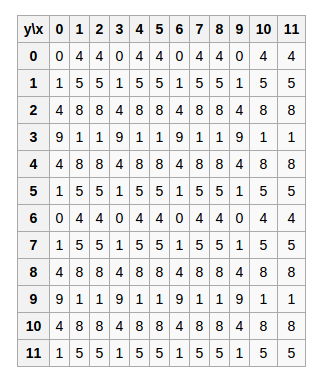
\includegraphics[scale=0.5]{2.png}
		\caption{Tabla de ejemplo de la primera restricción del algoritmo} 
	\end{center}
\end{figure}
\pagebreak
\begin{figure}[h]
	\begin{center}
		\[3x^{2}+y^{2}\]
		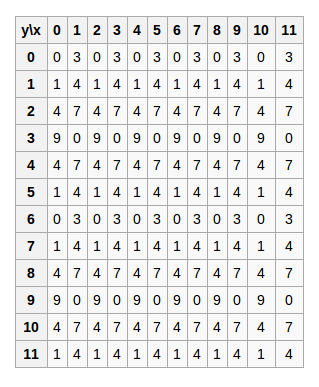
\includegraphics[scale=0.5]{3.png}
		\caption{Tabla de ejemplo de la segunda restricción del algoritmo} 
	\end{center}
\end{figure}

\begin{figure}[h]
	\begin{center}
		\[3x^{2}-y^{2}\]
		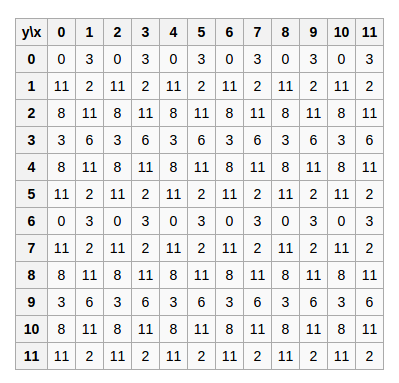
\includegraphics[scale=0.5]{4.png}
		\caption{Tabla de ejemplo de la tercera restricción del algoritmo} 
	\end{center}
\end{figure}
\subsection{Test de Solovay-Strassen}
Supongamos que $n$ es un entero positivo impar y queremos saber si $n$ es un numero primo o compuesto. Para ello se eligen $k$ enteros $0<b<n$ aleatoriamente. Para cada uno de estos números $b$ se calculan los valores de $b^{(n-1)/2}$ y de $\frac{b}{n}$.\cite{d}

\

Si estos valores no son congruentes modulo $n$, entonces $n$ es un numero compuesto y el test se detiene. en otro caso, se prueba el siguiente valor de $b$. Si los valores aleatoriamente calculados son congruentes para $k$ valores de $b$, independientemente elegidos, entonces hay una probabilidad menor a $2^{-k}$ de que $n$ no sea primo.

\

Si $n$ es un numero entero par y $b$ es un entero con $mcd(n,b) = 1 $ y se verifica la congruencia anterior, entonces n se llama un pseudoprimo de Euler base b.

Donde:
\begin{equation}
\left( \frac{b}{n} \right) = \left\{ \begin{array}{l}
0\ si\ n\ divide\ a\ b\\		
1\ si\ b\ es\ un\ residuo\ cuadratico\ 
modulo\ n \\
-1\ si\ b\ no\ es\ un\ residuo\ cuadratico\ modulo\ n 
\end{array}
\right.	
\end{equation}

Sea $a\in Z$ y $p$ es primo, $p>2$, diremos que $a$ es un residuo cuadrático $(mod\ p)$, si y solo si existe $x\in Z$ tal que $x\equiv a(p)$.


Por lo que para cualquier número $n$ que sea entero e impar, la probabilidad de error es de  $(\frac{1}{2})^{t}$   
\subsection{Teorema de Miller-Rabin}
La primera propuesta fue dada por G. L. Miller, que desde un inicio se trataba de un algoritmo determinista de Riemann. Lo que hizo Oser Rabin fue modificar la propuesta de Miller y de esta modificación obtuvo un algoritmo probabilístico.\cite{f}

\

Dado $n$ un primo mayor a un numero impar del cual queremos saber si es primo o no. Sea $m$ un valor impar tal que $n-1 = 2^{k} m$ y a tal que $2\leq a\leq n - 2$, Cuando se cumple:
\begin{center}
	$a^{m}\equiv 1\ mod\ n$
	
	o
	
	$a^{2m}\equiv-1\ mod\ n$
\end{center}

Para al menos un $r$ entero tal que $1\leq r\leq k-1$, se considera que $n$ es un probable primo; en caso contrario $n$ no puede ser primo.

\

Por lo que para cualquier número $n$ que sea entero e impar, la probabilidad de error es de  $(\frac{1}{4})^{t}$  

Si comparamos este algoritmo con el anterior(Solovay-Strassen), tendremos que Miller - Rabin es mucho mejor en varios aspectos, y las razones son que:
\begin{enumerate}
	\item Solovay-Strassen es mucho mas caro(computacionalmente hablando) que Miller-Rabin. 
	\item También que la probabilidad de error de Solovay-Strassen ($(\frac{1}{2})^{t}$) es mucho mas alta que la de Miller-Rabin ($(\frac{1}{4})^{t}$)
\end{enumerate}

\subsection{Algoritmo de Williams/Schmid}
En 1979, Williams y Schmid propusieron el siguiente algoritmo, es efectivo y altamente recomendado para generar primos fuertes.

\begin{enumerate}
	\item Encontrar dos primos $P''$ y $P^{+}$ del tamaño de bits elegido.
	\item Calcular $R=-(P'')^{-1}mod\ P^{+}$
	Por tanto $0 < r < P^{+}$, La inversa de $P''$ en modulo $P^{m}$ puede ser	calculada mediante el algoritmo extendido de Euclides.
	\item Encontrar el menor A tal que
	
	\begin{center}
		$P' = 2AP''P^{+}+2RP''+1,y$
		
		$P=4AP^{n}P^{+}+4AP''+3$	
	\end{center}
	O encontrado $P'$
	\begin{center}
		$P=2P'+1$	
	\end{center}
	Hasta que sean primos
\end{enumerate}
\subsection{Algoritmo de Gordon}
En 1984, John Gordon y propuso un nuevo algoritmo para generar primos fuertes, este es un poco mas eficiente que el de Williams/Schmid, debido a que no necesita calcular un $P'$ fuerte.

\textbf{Algoritmo}
\begin{enumerate}
	\item Encontrar dos primos $P''$ y $P^{+}$ del tamaño de bits elegido.
	\item Calcular el menor primo de la forma $P' = A''P'' + 1$ para algún entero $A''$
	\item Dejar
	\begin{center}
		$P_{0} = ((P^{+})^{P'-1}-(P')^{P^{+}-1})(P'P^{++})$
	\end{center}
	
	Notar que esto por el teorema de Fermat implicaría que $P' \equiv 1(mod\ P')$ y $P' \equiv -1 (mod\ p+)$
	
	\item Calcular el menor primo P de la siguiente manera
	\begin{center}
		$P_{0}=+AP'P^{+}$	
	\end{center}
	para algun entero $A$.
\end{enumerate}

\subsection{Espiral de Ulam}
La espiral de Ulam, descrita por el matemático polaco-estadounidense Stanis law Marcin Ulam (1909-1984), es una forma de representación gráfica de números primos que muestra un patrón.

\

Todos los números primos, excepto el 2, son impares. Como en la espiral de Ulam algunas diagonales contienen números impares y otras contienen números pares, no sorprende ver como los números primos caen todos (salvo el 2) en diagonales alternas. Sin embargo, entre las diagonales que contienen números impares, unas contienen una proporción visiblemente mayor que otras de números primos.

\

Las pruebas que se han hecho hasta ahora confirman que: incluso si se extiende mucho la espiral, se siguen mostrando esas diagonales; El patrón se muestra igualmente aunque el numero central no sea 1 (en efecto, puede ser mucho mayor que 1). Esto significa que hay muchas constantes enteras b y c tales que la función:

\begin{center}
	$f(n) = 4n^{2} + bn + c$
\end{center}
\subsection{Test de Lucas}
$M_{p}$ es primo si y solo si, $\frac{U_{2^{p}}}{U_{2^{p-1}}} \equiv 0 (mod\  M_{p})$

Con $U_{n}$ = termino n-ésimo de la sucesión de Fibonacci
Sucesión de Fibonacci:\{1, 1, 2, 3, 5, 8, 13, 21,...\}

\subsection{Test de Jacobi Sum}
Es un test basada en la idea de congruencia de conjuntos, cada uno con una analogía a el teorema de Fermat. El tiempo de ejecución determinado por un entero $n$ es \[O((ln\ n)^{c\ ln\ ln\ ln\ n})\] en operaciones de bits por algún constante $c$. Este es casi un algoritmo polinómico ya que el exponente $ln( ln( ln(n)))$ actúa como una una constante para un rango de valores $n$ de interés.\cite{g}

\

\textbf{Ejemplo.} Si $n \leq 2^{512}$, entonces $ln(ln(ln(n)))<1.78$.

\

La versión de Jacobi, usado en la practica es un algoritmo aleatorio que termina dentro de $O((ln\ n)^{c\ ln\ ln\ ln\ n})$ pasos con una probabilidad de al menos $1-(\frac{1}{2})^{k}$ por cada $k \geq 1$ y siempre tienes una respuesta correcta. 

\

Un inconveniente del algoritmo es que no produce un <<certificado>> que permitiría a la respuesta verificarse en el tiempo mucho más corto que ejecuta el propio algoritmo.

\

El test de Jacobi sum es, de hecho, práctico en el sentido de que la primalidad de los números que son varios cientos de dígitos decimales larga se pueden manejar en tan sólo unos minutos en un equipo. Sin embargo, la prueba no es tan fácil de programar como la prueba de Miller-Rabin probabilístico, y el código resultante no es tan compacto. Los detalles del algoritmo son complicados .

\section{Conclusión}
Para mi conclusión terminaré escogiendo un test pero antes de eso tengo que presentar los dos posibles candidatos que me han atraído mucho, estos son el test de Jacobi Sum y el teorema de Miller-Rabin.

\

El test de Jacobi Sum, me interesa mucho porque  la complejidad algorítmica que traza este algoritmo que es de:
\[O((ln\ n)^{c\ ln\ ln\ ln\ n})\]

Esto significa que la prueba de Jacobi sum resultante es bastante eficiente y logra los resultados de forma muy rápida a comparación de los otros algoritmos que hemos visto.

\

Pero cabe recalcar como ya hemos dicho anterior mente que el test de Jacobi Sum no proporciona un certificado de que el $n$(el número a probar) sea un numero primo al 100\%, por lo que la única manera de comprobar computacionalmente es volverlo a realizar el mismo proceso de comprobación varias veces para tener un rango mas alto de probabilidad de que es un número primo.

\

Bueno, pero desde el punto de vista del teorema de Miller - Rabin parece ser mucho más rápido que el de Jacobi sum, pero mejor veamoslo en la siguiente tabla:

\begin{figure}[h]
	\begin{center}
		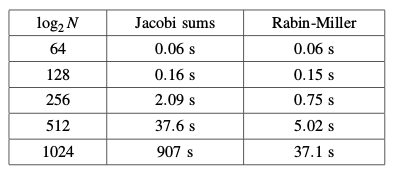
\includegraphics[scale=0.6]{7.png}
		\caption{Test de Jacobi sum y Rabin Miller} 
	\end{center}
\end{figure}

Esta tabla nos presenta una progresión algorítmica muy significativa. Para ser honesto cuando descubrí esto me que de atónito ya que pensaba que Jacobi test era mucho mejor.\cite{h}

\

Sucede que dentro de la complejidad algorítmica de Jacobi test $(ln\ n)^{c}$ podemos apreciar que $c$ vendría a ser uno de los primeros problemas que se presentan para este algoritmo ya que ya sea cualquier base que tenga siempre se va a elevar $c$ veces.

\

Para un entendimiento mejor de mi punto de vista esta esta gráfica:

\begin{figure}[h]
	\begin{center}
		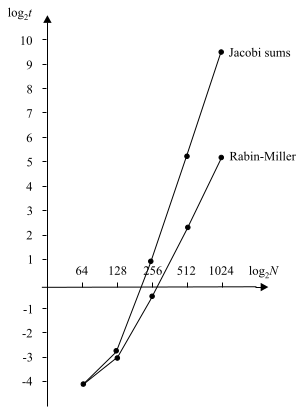
\includegraphics[scale=0.8]{8.png}
		\caption{Comparaciones de tiempo de respuesta.} 
	\end{center}
\end{figure}

Desde esta gráfica comparativa podemos ver mucho mejor como es que la velocidad influyen en ambos algoritmos.

\

Sin duda me quedo con el algritmo de Miller - Rabin por razones muy obvias.

\onecolumn

\bibliographystyle{plain}
\bibliography{biblio.bib}
\end{document}